\documentclass[tikz,border=15pt,12pt]{standalone}
\usepackage{fontawesome5}
\usepackage{enumitem}
\usepackage{xcolor}

\usetikzlibrary{shapes.geometric, arrows.meta, positioning, calc, backgrounds}

% Define colors matching the reference
\definecolor{box1border}{HTML}{296791}
\definecolor{box1top}{HTML}{E3F1FA}
\definecolor{box2border}{HTML}{3C8E47}
\definecolor{box2top}{HTML}{E6F7E9}
\definecolor{box3border}{HTML}{CB8124}
\definecolor{box3top}{HTML}{FAEBDA}
\definecolor{box4border}{HTML}{B72D37}
\definecolor{box4top}{HTML}{F9DFE0}
\definecolor{boxbot}{HTML}{FFFFFF}

\tikzset{
    basebox/.style args={#1/#2}{
        rectangle, 
        rounded corners=8pt,
        minimum width=4.4cm,
        minimum height=8.4cm,
        line width=1.3pt,
        draw=#1,
        path picture={
            % Fill total with bottom color
            \fill[boxbot] (path picture bounding box.south west) rectangle (path picture bounding box.north east);
            % Fill top with top color
            \fill[#2] (path picture bounding box.north west) rectangle ([yshift=-2.8cm]path picture bounding box.north east);
            % Draw separator line
            \draw[#1, opacity=0.4, line width=0.8pt] ([yshift=-2.8cm]path picture bounding box.north west) -- ([yshift=-2.8cm]path picture bounding box.north east);
        }
    },
    box1/.style={basebox=box1border/box1top},
    box2/.style={basebox=box2border/box2top},
    box3/.style={basebox=box3border/box3top},
    box4/.style={basebox=box4border/box4top},
    title/.style={
        font=\sffamily\bfseries\Large,
        align=left,
        text width=3.8cm
    },
    icon/.style={
        font=\fontsize{24}{28}\selectfont
    },
    bullettext/.style={
        font=\sffamily\normalsize,
        align=left,
        text width=3.8cm,
        text=black!85
    },
    arrowline/.style={
        draw, 
        -{Stealth[scale=0.9, width=2.5mm, length=3mm]}, 
        line width=1.5pt
    }
}

\begin{document}
\begin{tikzpicture}[node distance=0.6cm]

% Background grid
\begin{scope}[on background layer]
    \draw[step=1cm, gray!15, very thin] (-2.5,-9.0) grid (20.5,1.5);
\end{scope}

% Box 1 Base
\node[box1] (b1) at (0,-4.2) {};
\node[icon, text=box1border, anchor=north west] (i1) at ([shift={(0.3cm,-0.4cm)}]b1.north west) {\faSearch};
\node[title, text=box1border, anchor=north west] (t1) at ([shift={(0.3cm,-1.2cm)}]b1.north west) {Stage 1:\\Systematic\\Mapping Study};
\node[bullettext, anchor=north west] (l1) at ([shift={(0.3cm,-3.0cm)}]b1.north west) {
\begin{itemize}[leftmargin=10pt, topsep=0pt, itemsep=2pt, parsep=2pt, label={-}]
    \item Collect and\\analyze existing\\literature
    \item Identify key\\research trends\\and gaps
    \item Classify prior\\work
\end{itemize}
};

% Box 2 Base
\node[box2, right=of b1] (b2) {};
\node[icon, text=box2border, anchor=north west] (i2) at ([shift={(0.3cm,-0.4cm)}]b2.north west) {\faCog~\faFlask}; 
\node[title, text=box2border, anchor=north west] (t2) at ([shift={(0.3cm,-1.2cm)}]b2.north west) {Stage 2:\\Experimental\\Feasibility};
\node[bullettext, anchor=north west] (l2) at ([shift={(0.3cm,-3.0cm)}]b2.north west) {
\begin{itemize}[leftmargin=10pt, topsep=0pt, itemsep=2pt, parsep=2pt, label={-}]
    \item Develop initial\\prototypes
    \item Conduct\\proof-of-concept\\experiments
    \item Assess\\technical\\viability
\end{itemize}
};

% Box 3 Base
\node[box3, right=of b2] (b3) {};
\node[icon, text=box3border, anchor=north west] (i3) at ([shift={(0.3cm,-0.4cm)}]b3.north west) {\faSitemap};
\node[title, text=box3border, anchor=north west] (t3) at ([shift={(0.3cm,-1.2cm)}]b3.north west) {Stage 3:\\Cart-OnePiece\\Framework};
\node[bullettext, anchor=north west] (l3) at ([shift={(0.3cm,-3.0cm)}]b3.north west) {
\begin{itemize}[leftmargin=10pt, topsep=0pt, itemsep=2pt, parsep=2pt, label={-}]
    \item Propose new\\theoretical\\model
    \item Implement the\\Cart-OnePiece\\system
    \item Integrate\\components\\and protocols
\end{itemize}
};

% Box 4 Base
\node[box4, right=of b3] (b4) {};
\node[icon, text=box4border, anchor=north west] (i4) at ([shift={(0.3cm,-0.4cm)}]b4.north west) {\faChartBar};
\node[title, text=box4border, anchor=north west] (t4) at ([shift={(0.3cm,-1.2cm)}]b4.north west) {Stage 4:\\Empirical\\Evaluation};
\node[bullettext, anchor=north west] (l4) at ([shift={(0.3cm,-3.0cm)}]b4.north west) {
\begin{itemize}[leftmargin=10pt, topsep=0pt, itemsep=2pt, parsep=2pt, label={-}]
    \item Execute\\controlled\\experiments
    \item Compare with\\baseline\\methods
    \item Analyze\\quantitative\\performance\\data
\end{itemize}
};

% Arrows
\draw[arrowline, box1border] (b1.east) -- (b2.west);
\draw[arrowline, box2border] (b2.east) -- (b3.west);
\draw[arrowline, box3border] (b3.east) -- (b4.west);

\end{tikzpicture}
\end{document}
